\SourceLeaf{218}%
Ebene, deren Durchschnitte das Dreieck $ABC$ bilden, so geben die drei Winkelpunkte uns die Gleichungen:

\[ 2a + 2\alpha = 4R, \]
\[ 2b + 2\beta = 4R, \]
\[ 2c + 2\gamma = 4R, \]

\noindent also

\[ \alpha + \beta + \gamma = 6R - (a+b+c). \]

Da diese Relationen bestehen, wie auch die Punkte $A$, $B$, $C$ liegen mögen, oder, was einerlei ist, wie auch die drei Linien im Raume gezogen sind, so lasse man die Linien $\overline{DG}$, $\overline{EH}$ unverrückt, und ziehe $\overline{JF}$ durch den Punkt $A$, so dass sie denselben Winkel als in ihrer vorigen Lage mit $EH$ macht oder, da

\begin{center}
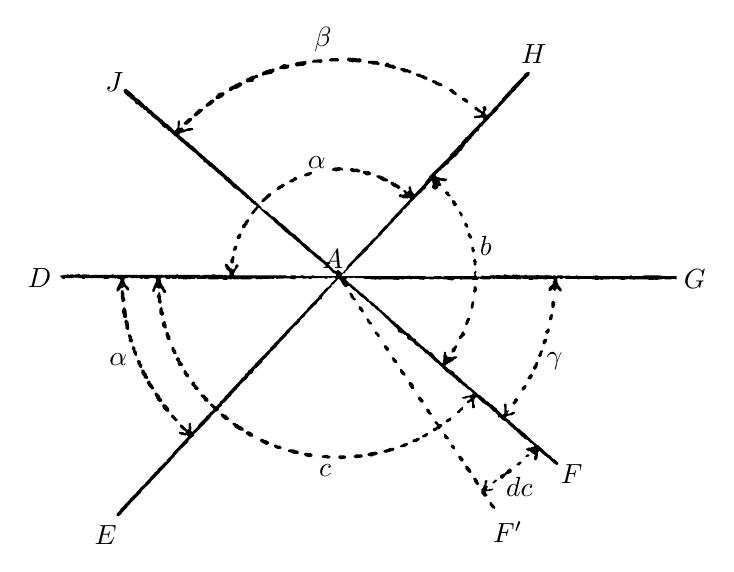
\begin{tikzpicture}[x=0.00698216cm,y=-0.00698216cm]
\fill[even odd rule] (870,876) -- (869,877) -- (869,881) -- (874,887) -- (878,888) -- (879,887) -- (879,884) -- (872,876) -- cycle
(864,836) -- (862,836) -- (860,838) -- (860,844) -- (858,846) -- (857,850) -- (854,853) -- (854,860) -- (859,866) -- (862,866) -- (865,864) -- (865,862) -- (862,859) -- (862,857) -- (863,856) -- (869,856) -- (870,855) -- (873,855) -- (876,852) -- (875,851) -- (873,852) -- (868,852) -- (867,853) -- (865,853) -- (864,852) -- (864,850) -- (866,848) -- (863,845) -- (863,843) -- (865,839) -- (865,837) -- cycle
(882,836) -- (881,835) -- (879,835) -- (874,840) -- (874,841) -- (875,842) -- (878,841) -- (882,837) -- cycle
(840,832) -- (839,834) -- (840,835) -- (841,839) -- (845,844) -- (848,845) -- (850,842) -- (850,841) -- (848,839) -- (848,837) -- (844,832) -- cycle
(909,817) -- (907,815) -- (904,815) -- (896,824) -- (894,824) -- (890,826) -- (888,828) -- (888,831) -- (890,833) -- (893,833) -- (899,826) -- (907,823) -- (909,821) -- cycle
(826,810) -- (825,811) -- (825,815) -- (826,817) -- (831,822) -- (834,823) -- (836,821) -- (835,817) -- (829,810) -- cycle
(927,804) -- (925,802) -- (922,803) -- (918,807) -- (918,808) -- (919,809) -- (923,809) -- (927,805) -- cycle
(813,792) -- (812,793) -- (812,796) -- (814,798) -- (814,799) -- (817,802) -- (820,802) -- (822,798) -- (817,792) -- cycle
(594,793) -- (594,795) -- (598,798) -- (606,797) -- (608,795) -- (608,793) -- (605,791) -- (596,791) -- cycle
(564,792) -- (564,794) -- (565,795) -- (567,795) -- (568,796) -- (573,796) -- (574,797) -- (576,797) -- (580,794) -- (579,792) -- (575,791) -- (574,790) -- (569,790) -- (568,791) -- (565,791) -- cycle
(941,790) -- (940,789) -- (937,789) -- (934,792) -- (934,793) -- (935,794) -- (940,793) -- (941,792) -- cycle
(622,792) -- (622,793) -- (625,796) -- (636,795) -- (638,793) -- (638,791) -- (636,789) -- (626,789) -- cycle
(532,788) -- (532,790) -- (535,793) -- (538,793) -- (539,794) -- (544,794) -- (547,792) -- (547,789) -- (544,787) -- (538,787) -- (537,786) -- (535,786) -- cycle
(666,787) -- (664,785) -- (659,784) -- (658,785) -- (653,785) -- (652,786) -- (650,786) -- (647,789) -- (647,790) -- (649,792) -- (655,793) -- (659,791) -- (662,791) -- (664,789) -- (665,789) -- cycle
(503,782) -- (503,784) -- (504,785) -- (506,785) -- (513,788) -- (521,788) -- (522,787) -- (522,784) -- (519,782) -- (516,782) -- (513,780) -- (505,780) -- cycle
(696,779) -- (694,777) -- (686,778) -- (685,779) -- (678,781) -- (676,783) -- (676,784) -- (678,786) -- (683,786) -- (684,785) -- (687,785) -- (690,783) -- (693,783) -- (696,780) -- cycle
(800,771) -- (798,775) -- (802,779) -- (805,780) -- (806,779) -- (806,775) -- (803,772) -- cycle
(477,773) -- (477,775) -- (479,777) -- (483,779) -- (489,779) -- (491,777) -- (491,776) -- (488,773) -- (484,773) -- (479,771) -- cycle
(721,770) -- (718,768) -- (716,769) -- (713,769) -- (711,771) -- (708,772) -- (706,774) -- (706,775) -- (707,776) -- (714,776) -- (719,773) -- (721,771) -- cycle
(452,763) -- (452,765) -- (454,767) -- (463,772) -- (466,771) -- (468,769) -- (468,767) -- (466,765) -- (462,763) -- (460,763) -- (457,761) -- (454,761) -- cycle
(742,760) -- (741,759) -- (737,759) -- (734,761) -- (732,761) -- (729,763) -- (729,766) -- (730,767) -- (735,767) -- (739,765) -- (742,762) -- cycle
(787,752) -- (786,753) -- (786,757) -- (787,759) -- (789,761) -- (793,762) -- (795,760) -- (795,759) -- (790,753) -- cycle
(757,751) -- (756,750) -- (754,750) -- (750,753) -- (747,754) -- (746,756) -- (748,758) -- (752,758) -- (757,754) -- cycle
(426,749) -- (426,752) -- (433,757) -- (438,757) -- (439,756) -- (439,752) -- (434,748) -- (430,747) -- cycle
(402,733) -- (402,735) -- (405,738) -- (405,739) -- (407,741) -- (410,742) -- (413,745) -- (415,745) -- (416,746) -- (421,746) -- (422,745) -- (422,742) -- (419,739) -- (414,737) -- (411,734) -- (409,734) -- (407,732) -- (403,732) -- cycle
(773,729) -- (770,729) -- (769,730) -- (769,732) -- (773,736) -- (773,738) -- (770,741) -- (768,741) -- (766,743) -- (766,745) -- (768,747) -- (772,746) -- (775,743) -- (778,743) -- (783,737) -- (783,736) -- (781,734) -- (777,734) -- cycle
(798,722) -- (792,725) -- (789,728) -- (789,729) -- (791,731) -- (793,731) -- (799,727) -- (799,723) -- cycle
(292,717) -- (290,719) -- (290,721) -- (298,729) -- (301,728) -- (302,727) -- (302,725) -- (300,724) -- (294,717) -- cycle
(380,716) -- (382,721) -- (388,726) -- (392,727) -- (395,725) -- (395,723) -- (389,717) -- (387,717) -- (385,715) -- (381,715) -- cycle
(755,706) -- (754,707) -- (754,711) -- (759,717) -- (763,717) -- (764,715) -- (761,711) -- (761,709) -- (759,707) -- cycle
(820,703) -- (819,703) -- (810,711) -- (810,713) -- (811,714) -- (814,714) -- (816,712) -- (816,711) -- (820,708) -- (821,706) -- (821,704) -- cycle
(276,698) -- (274,700) -- (275,705) -- (281,711) -- (285,712) -- (287,709) -- (286,705) -- (281,699) -- (279,698) -- cycle
(920,688) -- (917,687) -- (914,689) -- (913,692) -- (911,694) -- (911,697) -- (912,698) -- (915,698) -- (918,695) -- (921,690) -- cycle
(741,684) -- (739,686) -- (739,689) -- (744,695) -- (747,695) -- (749,693) -- (749,691) -- (743,684) -- cycle
(346,680) -- (344,682) -- (344,683) -- (349,688) -- (350,691) -- (352,693) -- (357,693) -- (358,692) -- (358,689) -- (357,687) -- (351,681) -- cycle
(262,677) -- (260,679) -- (260,680) -- (261,681) -- (261,683) -- (263,685) -- (263,687) -- (265,689) -- (265,691) -- (269,694) -- (273,693) -- (274,692) -- (274,689) -- (270,685) -- (270,683) -- (264,677) -- cycle
(934,663) -- (933,663) -- (927,668) -- (927,672) -- (928,673) -- (931,673) -- (935,669) -- (936,665) -- cycle
(723,658) -- (722,659) -- (722,662) -- (724,666) -- (727,670) -- (731,670) -- (732,669) -- (731,663) -- (728,659) -- (726,658) -- cycle
(330,657) -- (327,660) -- (327,663) -- (331,667) -- (334,672) -- (338,672) -- (340,670) -- (340,668) -- (334,662) -- (333,658) -- (332,657) -- cycle
(249,655) -- (246,658) -- (246,659) -- (249,665) -- (255,671) -- (257,671) -- (259,669) -- (259,667) -- (257,665) -- (256,662) -- (253,659) -- (253,657) -- (251,655) -- cycle
(945,643) -- (942,644) -- (940,646) -- (940,647) -- (938,649) -- (938,651) -- (939,652) -- (943,653) -- (946,650) -- (947,648) -- (947,645) -- cycle
(315,636) -- (313,638) -- (313,642) -- (317,648) -- (321,649) -- (323,646) -- (323,644) -- (319,640) -- (319,639) -- (316,636) -- cycle
(237,635) -- (236,636) -- (236,641) -- (238,645) -- (240,647) -- (240,649) -- (242,651) -- (247,652) -- (248,651) -- (248,648) -- (246,645) -- (246,643) -- (243,640) -- (242,637) -- (240,635) -- cycle
(707,634) -- (706,635) -- (707,641) -- (711,645) -- (715,646) -- (716,645) -- (716,642) -- (709,634) -- cycle
(955,621) -- (954,621) -- (952,623) -- (951,626) -- (948,630) -- (948,633) -- (950,635) -- (952,635) -- (954,633) -- (956,629) -- (957,623) -- cycle
(230,618) -- (228,620) -- (229,622) -- (229,625) -- (231,627) -- (231,629) -- (234,632) -- (236,632) -- (237,631) -- (238,627) -- (235,623) -- (235,620) -- (232,618) -- cycle
(692,613) -- (691,615) -- (692,616) -- (693,620) -- (697,623) -- (700,623) -- (701,622) -- (701,619) -- (695,613) -- cycle
(301,613) -- (299,615) -- (299,618) -- (302,621) -- (302,625) -- (304,628) -- (310,629) -- (312,625) -- (308,621) -- (306,617) -- (306,615) -- (304,613) -- cycle
(965,600) -- (962,600) -- (960,602) -- (959,606) -- (957,609) -- (957,610) -- (959,612) -- (961,612) -- (964,609) -- (964,606) -- (966,602) -- cycle
(292,594) -- (291,595) -- (291,600) -- (295,607) -- (299,607) -- (300,606) -- (299,600) -- (296,597) -- (296,595) -- (295,594) -- cycle
(220,593) -- (219,594) -- (219,598) -- (221,600) -- (221,603) -- (223,607) -- (226,610) -- (227,610) -- (228,609) -- (228,603) -- (225,599) -- (225,595) -- (223,593) -- cycle
(809,591) -- (807,591) -- (801,597) -- (800,599) -- (800,603) -- (801,604) -- (805,603) -- (807,601) -- (808,597) -- (810,595) -- (810,592) -- cycle
(678,591) -- (677,592) -- (677,594) -- (679,598) -- (682,601) -- (684,601) -- (686,599) -- (686,596) -- (681,591) -- cycle
(972,579) -- (969,579) -- (966,582) -- (965,587) -- (967,589) -- (969,589) -- (972,586) -- (973,584) -- (973,580) -- cycle
(213,571) -- (212,572) -- (212,575) -- (213,576) -- (213,579) -- (214,580) -- (213,583) -- (215,585) -- (219,586) -- (221,583) -- (220,579) -- (219,578) -- (219,575) -- (216,571) -- cycle
(282,567) -- (280,570) -- (280,573) -- (281,574) -- (282,579) -- (284,581) -- (288,581) -- (289,580) -- (289,575) -- (286,571) -- (286,569) -- (284,567) -- cycle
(822,566) -- (819,566) -- (816,572) -- (813,575) -- (813,578) -- (814,579) -- (817,579) -- (823,573) -- (825,572) -- cycle
(661,566) -- (660,567) -- (661,570) -- (666,576) -- (668,576) -- (669,575) -- (669,571) -- (664,566) -- cycle
(976,560) -- (975,560) -- (970,565) -- (970,567) -- (973,570) -- (976,569) -- (978,566) -- (978,562) -- cycle
(277,547) -- (274,550) -- (274,556) -- (278,560) -- (281,560) -- (282,559) -- (282,554) -- (281,553) -- (280,548) -- (279,547) -- cycle
(208,544) -- (205,548) -- (206,550) -- (206,553) -- (207,554) -- (207,560) -- (210,563) -- (212,563) -- (214,561) -- (214,553) -- (213,552) -- (213,549) -- (212,547) -- (209,544) -- cycle
(647,542) -- (645,544) -- (647,549) -- (651,553) -- (654,553) -- (655,552) -- (655,550) -- (651,546) -- (651,545) -- (648,542) -- cycle
(832,541) -- (829,541) -- (826,546) -- (826,548) -- (825,549) -- (825,553) -- (826,554) -- (828,554) -- (831,550) -- (831,548) -- (833,545) -- (833,542) -- cycle
(982,534) -- (978,536) -- (978,539) -- (977,540) -- (977,544) -- (978,545) -- (981,545) -- (983,543) -- (984,536) -- cycle
(204,522) -- (201,527) -- (201,532) -- (202,533) -- (203,539) -- (205,541) -- (208,541) -- (210,539) -- (209,527) -- (206,522) -- cycle
(272,521) -- (269,525) -- (269,533) -- (272,537) -- (274,537) -- (277,535) -- (277,531) -- (276,530) -- (274,522) -- cycle
(632,520) -- (631,521) -- (631,524) -- (632,526) -- (637,531) -- (639,531) -- (640,530) -- (640,527) -- (636,521) -- cycle
(840,511) -- (838,511) -- (836,513) -- (836,516) -- (835,517) -- (835,523) -- (836,524) -- (838,524) -- (840,521) -- (840,517) -- (841,516) -- (841,512) -- cycle
(985,510) -- (984,510) -- (981,513) -- (981,521) -- (983,523) -- (985,523) -- (988,519) -- (988,513) -- cycle
(616,495) -- (614,497) -- (614,498) -- (616,500) -- (616,503) -- (622,509) -- (625,509) -- (626,507) -- (623,504) -- (620,498) -- (617,495) -- cycle
(268,494) -- (264,502) -- (266,506) -- (266,512) -- (269,515) -- (271,515) -- (273,513) -- (273,510) -- (272,509) -- (271,498) -- (270,497) -- (270,495) -- cycle
(200,491) -- (199,492) -- (199,507) -- (200,508) -- (200,511) -- (201,512) -- (204,512) -- (207,509) -- (207,507) -- (205,503) -- (205,496) -- (204,495) -- (204,492) -- (203,491) -- cycle
(841,484) -- (840,485) -- (840,490) -- (839,491) -- (839,493) -- (841,495) -- (843,495) -- (846,491) -- (846,487) -- (844,484) -- cycle
(841,434) -- (839,437) -- (839,439) -- (840,440) -- (840,444) -- (842,446) -- (843,446) -- (845,444) -- (845,441) -- (846,439) -- (844,437) -- (844,435) -- (843,434) -- cycle
(404,429) -- (402,429) -- (400,431) -- (400,433) -- (398,435) -- (398,440) -- (400,442) -- (402,442) -- (404,440) -- (404,437) -- (405,436) -- (405,430) -- cycle
(837,412) -- (836,413) -- (836,418) -- (837,420) -- (839,422) -- (840,422) -- (842,419) -- (842,417) -- (841,416) -- (841,414) -- (839,412) -- cycle
(409,410) -- (406,410) -- (404,412) -- (403,416) -- (402,417) -- (403,419) -- (407,419) -- (409,417) -- (410,415) -- (410,411) -- cycle
(417,388) -- (414,388) -- (410,392) -- (409,395) -- (411,398) -- (414,398) -- (417,395) -- (417,392) -- (418,391) -- (418,389) -- cycle
(831,387) -- (829,389) -- (829,392) -- (833,397) -- (835,397) -- (837,395) -- (837,393) -- (833,387) -- cycle
(825,368) -- (823,370) -- (823,373) -- (827,377) -- (829,377) -- (830,376) -- (830,372) -- (826,368) -- cycle
(431,362) -- (428,362) -- (425,365) -- (423,369) -- (419,373) -- (419,377) -- (420,378) -- (424,378) -- (425,377) -- (426,374) -- (429,371) -- (429,369) -- (432,366) -- (432,363) -- cycle
(814,348) -- (813,349) -- (813,351) -- (815,353) -- (816,356) -- (818,357) -- (820,355) -- (820,352) -- (816,348) -- cycle
(802,327) -- (801,328) -- (801,333) -- (802,334) -- (802,336) -- (805,338) -- (807,338) -- (810,335) -- (810,334) -- (808,332) -- (806,328) -- cycle
(472,316) -- (471,315) -- (467,315) -- (459,323) -- (457,324) -- (454,329) -- (455,330) -- (459,330) -- (472,319) -- cycle
(788,313) -- (788,315) -- (793,320) -- (797,320) -- (798,319) -- (798,318) -- (795,315) -- (795,313) -- (794,312) -- (791,311) -- cycle
(497,300) -- (495,298) -- (492,297) -- (489,300) -- (486,301) -- (482,305) -- (482,307) -- (484,309) -- (489,307) -- (491,305) -- (493,305) -- (497,301) -- cycle
(689,295) -- (689,298) -- (696,304) -- (699,304) -- (703,307) -- (704,307) -- (707,304) -- (707,303) -- (703,299) -- (700,298) -- (698,296) -- (696,296) -- (694,294) -- (690,294) -- cycle
(519,287) -- (517,285) -- (514,285) -- (511,288) -- (507,290) -- (505,292) -- (505,294) -- (506,295) -- (512,295) -- (515,292) -- (519,290) -- cycle
(663,283) -- (663,284) -- (667,288) -- (669,288) -- (671,290) -- (677,293) -- (683,293) -- (684,292) -- (684,290) -- (682,288) -- (679,287) -- (676,284) -- (674,284) -- (670,282) -- (664,282) -- cycle
(546,277) -- (545,276) -- (541,276) -- (540,277) -- (538,277) -- (534,279) -- (532,281) -- (532,282) -- (534,284) -- (540,283) -- (544,281) -- (546,279) -- cycle
(639,275) -- (639,278) -- (645,282) -- (649,282) -- (653,280) -- (653,277) -- (649,274) -- (647,274) -- (646,275) -- (644,274) -- (640,274) -- cycle
(615,271) -- (615,273) -- (619,276) -- (629,276) -- (631,277) -- (634,274) -- (634,273) -- (632,271) -- (630,271) -- (629,270) -- (622,270) -- (621,269) -- (617,269) -- cycle
(582,271) -- (583,273) -- (587,274) -- (588,275) -- (592,275) -- (593,274) -- (596,274) -- (597,273) -- (602,273) -- (603,272) -- (601,268) -- (598,268) -- (597,267) -- (586,268) -- cycle
(328,179) -- (327,178) -- (323,178) -- (321,179) -- (313,187) -- (313,188) -- (315,190) -- (319,190) -- (328,182) -- cycle
(348,163) -- (346,161) -- (342,161) -- (340,162) -- (331,171) -- (331,172) -- (334,175) -- (336,175) -- (340,171) -- (341,171) -- (348,164) -- cycle
(369,146) -- (366,144) -- (362,145) -- (353,153) -- (353,156) -- (354,157) -- (357,157) -- (363,154) -- (368,149) -- cycle
(819,142) -- (819,145) -- (826,150) -- (829,150) -- (830,149) -- (830,146) -- (827,143) -- (823,141) -- (820,141) -- cycle
(387,133) -- (385,131) -- (377,132) -- (371,139) -- (371,142) -- (372,143) -- (377,143) -- (383,140) -- (387,136) -- cycle
(795,127) -- (795,128) -- (803,135) -- (805,135) -- (806,136) -- (808,136) -- (809,135) -- (809,132) -- (801,125) -- (798,125) -- cycle
(419,115) -- (417,113) -- (413,113) -- (411,115) -- (407,116) -- (404,119) -- (401,119) -- (399,121) -- (398,121) -- (395,124) -- (395,127) -- (397,129) -- (399,129) -- (405,125) -- (409,125) -- (416,121) -- (419,118) -- cycle
(764,111) -- (764,112) -- (767,115) -- (769,115) -- (772,118) -- (774,118) -- (777,120) -- (782,120) -- (783,119) -- (783,117) -- (781,115) -- (774,112) -- (772,110) -- (766,109) -- cycle
(448,101) -- (446,99) -- (445,99) -- (442,101) -- (438,101) -- (437,102) -- (435,102) -- (433,104) -- (429,105) -- (426,108) -- (426,111) -- (428,113) -- (439,112) -- (440,111) -- (440,109) -- (444,105) -- (447,105) -- (448,104) -- cycle
(735,98) -- (736,101) -- (739,103) -- (741,103) -- (751,108) -- (755,108) -- (756,107) -- (756,104) -- (749,100) -- (746,100) -- (742,97) -- (736,97) -- cycle
(1209,466) -- (1208,465) -- (1197,465) -- (1195,466) -- (1194,465) -- (1183,465) -- (1182,464) -- (1180,465) -- (1178,464) -- (1149,464) -- (1148,465) -- (1128,465) -- (1127,464) -- (1125,464) -- (1124,465) -- (1066,465) -- (1065,464) -- (1061,464) -- (1060,465) -- (1058,464) -- (1056,465) -- (1029,465) -- (1028,464) -- (1026,464) -- (1025,465) -- (1015,465) -- (1014,464) -- (1002,465) -- (1001,464) -- (992,464) -- (991,465) -- (989,465) -- (988,464) -- (985,464) -- (984,465) -- (982,465) -- (981,464) -- (975,464) -- (974,463) -- (972,463) -- (971,464) -- (959,464) -- (958,463) -- (954,463) -- (953,464) -- (937,464) -- (936,463) -- (933,463) -- (932,464) -- (924,464) -- (923,463) -- (919,463) -- (918,462) -- (916,463) -- (912,462) -- (909,464) -- (904,464) -- (903,463) -- (899,463) -- (898,462) -- (896,462) -- (894,464) -- (888,464) -- (887,463) -- (877,464) -- (875,463) -- (874,464) -- (870,464) -- (869,465) -- (858,465) -- (856,464) -- (853,466) -- (846,466) -- (844,464) -- (844,460) -- (845,459) -- (845,457) -- (844,456) -- (843,456) -- (841,458) -- (841,461) -- (842,463) -- (840,465) -- (787,465) -- (786,466) -- (782,466) -- (781,465) -- (769,465) -- (768,466) -- (753,466) -- (752,465) -- (725,465) -- (723,464) -- (722,465) -- (604,465) -- (602,466) -- (600,464) -- (600,463) -- (603,460) -- (606,460) -- (607,459) -- (607,457) -- (614,450) -- (614,449) -- (616,447) -- (617,447) -- (619,445) -- (619,444) -- (648,416) -- (650,412) -- (657,406) -- (657,405) -- (674,388) -- (674,387) -- (685,376) -- (685,375) -- (695,365) -- (695,364) -- (711,348) -- (711,346) -- (713,344) -- (714,344) -- (724,334) -- (724,333) -- (742,315) -- (743,315) -- (749,308) -- (750,308) -- (753,305) -- (753,303) -- (763,292) -- (765,293) -- (765,296) -- (766,297) -- (764,304) -- (767,307) -- (771,308) -- (775,305) -- (775,303) -- (777,301) -- (780,301) -- (781,300) -- (781,298) -- (778,294) -- (778,293) -- (780,291) -- (781,292) -- (785,292) -- (786,293) -- (788,293) -- (792,290) -- (791,288) -- (787,288) -- (786,287) -- (779,287) -- (778,286) -- (773,285) -- (771,283) -- (771,281) -- (779,273) -- (780,273) -- (784,268) -- (785,268) -- (790,263) -- (793,262) -- (795,260) -- (796,257) -- (805,249) -- (806,249) -- (812,243) -- (812,242) -- (816,237) -- (818,237) -- (822,230) -- (824,228) -- (825,225) -- (827,223) -- (828,223) -- (834,216) -- (836,215) -- (836,213) -- (841,208) -- (841,207) -- (846,202) -- (848,202) -- (849,201) -- (851,196) -- (854,193) -- (855,193) -- (857,191) -- (857,190) -- (869,178) -- (869,177) -- (871,175) -- (872,175) -- (874,173) -- (874,172) -- (882,165) -- (882,164) -- (885,161) -- (885,159) -- (898,146) -- (898,145) -- (908,135) -- (908,134) -- (917,126) -- (917,125) -- (931,110) -- (931,109) -- (941,100) -- (942,96) -- (940,94) -- (936,95) -- (933,97) -- (930,102) -- (908,124) -- (908,125) -- (901,132) -- (901,133) -- (897,136) -- (897,137) -- (892,142) -- (891,145) -- (885,151) -- (885,152) -- (880,157) -- (879,157) -- (872,165) -- (872,166) -- (865,172) -- (863,172) -- (861,170) -- (861,165) -- (863,163) -- (863,159) -- (861,156) -- (859,156) -- (856,159) -- (857,163) -- (858,164) -- (856,166) -- (855,166) -- (851,162) -- (850,162) -- (845,157) -- (841,159) -- (842,162) -- (844,164) -- (845,164) -- (848,167) -- (852,168) -- (854,170) -- (854,171) -- (852,173) -- (842,174) -- (841,175) -- (841,177) -- (842,178) -- (856,177) -- (858,179) -- (857,182) -- (852,187) -- (851,187) -- (849,189) -- (849,190) -- (840,199) -- (838,200) -- (838,201) -- (828,212) -- (826,212) -- (825,213) -- (825,214) -- (817,223) -- (817,225) -- (815,227) -- (814,227) -- (804,238) -- (802,239) -- (802,240) -- (797,245) -- (796,248) -- (760,283) -- (758,287) -- (752,294) -- (751,297) -- (733,316) -- (732,316) -- (729,313) -- (727,309) -- (726,303) -- (725,302) -- (723,302) -- (722,303) -- (722,307) -- (723,309) -- (720,312) -- (719,312) -- (716,309) -- (713,309) -- (712,311) -- (715,314) -- (715,315) -- (713,317) -- (709,317) -- (707,316) -- (704,318) -- (704,320) -- (706,322) -- (709,322) -- (712,324) -- (720,324) -- (721,323) -- (723,323) -- (724,324) -- (724,326) -- (689,363) -- (689,364) -- (684,369) -- (684,370) -- (682,372) -- (681,372) -- (667,387) -- (665,391) -- (661,395) -- (660,395) -- (652,403) -- (652,404) -- (637,418) -- (637,419) -- (625,431) -- (625,432) -- (611,446) -- (611,447) -- (609,449) -- (609,451) -- (601,460) -- (593,453) -- (593,454) -- (591,456) -- (587,455) -- (577,445) -- (577,444) -- (579,442) -- (580,442) -- (577,439) -- (576,440) -- (571,439) -- (567,435) -- (566,435) -- (561,429) -- (557,427) -- (549,420) -- (548,420) -- (542,414) -- (541,412) -- (540,412) -- (533,406) -- (532,406) -- (521,395) -- (520,395) -- (516,390) -- (509,386) -- (497,374) -- (496,374) -- (492,370) -- (488,368) -- (478,358) -- (473,356) -- (465,348) -- (456,343) -- (454,341) -- (454,340) -- (443,329) -- (442,329) -- (422,310) -- (421,310) -- (407,297) -- (406,297) -- (394,285) -- (393,285) -- (379,272) -- (378,272) -- (374,268) -- (373,268) -- (369,263) -- (368,263) -- (364,259) -- (363,259) -- (359,255) -- (358,255) -- (350,247) -- (349,247) -- (344,242) -- (343,242) -- (330,229) -- (326,227) -- (320,221) -- (319,221) -- (309,212) -- (308,212) -- (305,209) -- (305,207) -- (307,205) -- (313,204) -- (319,201) -- (325,201) -- (326,200) -- (329,200) -- (330,199) -- (330,197) -- (329,196) -- (322,196) -- (315,199) -- (313,199) -- (310,195) -- (306,196) -- (305,195) -- (305,192) -- (306,191) -- (306,183) -- (304,182) -- (302,185) -- (302,195) -- (300,197) -- (300,198) -- (297,201) -- (296,201) -- (285,190) -- (280,187) -- (273,180) -- (272,180) -- (267,175) -- (266,175) -- (262,171) -- (261,171) -- (253,163) -- (252,163) -- (245,156) -- (244,156) -- (233,145) -- (226,141) -- (224,139) -- (224,138) -- (213,128) -- (212,128) -- (209,125) -- (206,125) -- (204,127) -- (204,130) -- (205,132) -- (212,139) -- (213,139) -- (217,143) -- (221,145) -- (224,148) -- (225,151) -- (227,153) -- (230,153) -- (236,159) -- (238,159) -- (241,163) -- (243,163) -- (246,166) -- (246,167) -- (248,169) -- (252,171) -- (256,176) -- (257,176) -- (261,180) -- (264,181) -- (272,189) -- (275,194) -- (282,197) -- (285,201) -- (288,202) -- (296,210) -- (301,213) -- (304,217) -- (305,217) -- (310,222) -- (311,222) -- (319,230) -- (320,230) -- (329,238) -- (334,241) -- (346,253) -- (347,253) -- (349,255) -- (349,257) -- (350,258) -- (353,259) -- (360,266) -- (363,267) -- (376,279) -- (377,279) -- (382,284) -- (383,284) -- (386,287) -- (386,288) -- (396,297) -- (397,297) -- (404,305) -- (412,309) -- (429,325) -- (432,326) -- (437,332) -- (438,332) -- (441,335) -- (443,335) -- (445,337) -- (445,339) -- (436,349) -- (436,352) -- (437,353) -- (439,353) -- (443,349) -- (443,348) -- (447,344) -- (447,343) -- (449,341) -- (450,341) -- (461,352) -- (462,352) -- (467,357) -- (468,357) -- (473,362) -- (474,362) -- (480,369) -- (481,369) -- (486,374) -- (487,374) -- (499,386) -- (500,386) -- (505,391) -- (508,392) -- (514,398) -- (515,398) -- (520,403) -- (521,403) -- (539,420) -- (543,422) -- (556,434) -- (557,434) -- (564,440) -- (565,440) -- (571,446) -- (571,448) -- (572,449) -- (575,449) -- (585,460) -- (588,460) -- (591,463) -- (589,465) -- (550,465) -- (549,464) -- (546,464) -- (545,465) -- (532,465) -- (531,464) -- (526,464) -- (525,465) -- (518,465) -- (517,464) -- (508,464) -- (507,465) -- (500,465) -- (499,464) -- (406,464) -- (404,462) -- (404,461) -- (408,453) -- (413,447) -- (413,446) -- (411,444) -- (409,444) -- (407,446) -- (405,452) -- (404,453) -- (402,453) -- (400,451) -- (398,451) -- (392,443) -- (389,443) -- (388,444) -- (388,447) -- (391,453) -- (396,457) -- (396,460) -- (397,462) -- (395,464) -- (390,464) -- (389,463) -- (387,463) -- (386,464) -- (384,463) -- (371,463) -- (370,462) -- (365,462) -- (364,463) -- (349,463) -- (348,464) -- (343,464) -- (342,463) -- (303,463) -- (302,462) -- (300,462) -- (299,463) -- (279,463) -- (278,464) -- (276,463) -- (186,463) -- (185,462) -- (183,462) -- (182,463) -- (146,463) -- (144,464) -- (140,462) -- (138,463) -- (136,462) -- (129,462) -- (128,463) -- (126,463) -- (122,461) -- (121,462) -- (116,462) -- (115,463) -- (113,463) -- (112,462) -- (107,462) -- (106,463) -- (101,462) -- (100,463) -- (95,463) -- (94,464) -- (90,464) -- (89,465) -- (89,466) -- (93,470) -- (96,470) -- (97,469) -- (112,469) -- (113,468) -- (121,468) -- (122,469) -- (128,469) -- (129,470) -- (133,470) -- (134,469) -- (167,469) -- (168,470) -- (176,470) -- (177,469) -- (187,469) -- (189,470) -- (190,469) -- (192,469) -- (193,470) -- (196,470) -- (198,472) -- (198,474) -- (191,488) -- (191,492) -- (192,493) -- (194,493) -- (199,487) -- (202,487) -- (205,484) -- (210,491) -- (213,491) -- (214,490) -- (213,486) -- (207,480) -- (207,478) -- (205,475) -- (205,471) -- (207,469) -- (211,469) -- (212,468) -- (217,468) -- (218,469) -- (234,469) -- (235,470) -- (238,470) -- (239,469) -- (241,469) -- (242,470) -- (249,470) -- (250,469) -- (261,469) -- (263,471) -- (263,475) -- (260,480) -- (260,482) -- (258,484) -- (258,487) -- (256,489) -- (256,493) -- (257,494) -- (259,494) -- (261,491) -- (262,487) -- (263,486) -- (265,486) -- (267,488) -- (271,487) -- (274,490) -- (275,494) -- (278,496) -- (279,496) -- (281,494) -- (281,491) -- (278,488) -- (278,486) -- (275,483) -- (272,477) -- (271,470) -- (273,468) -- (279,468) -- (282,470) -- (288,470) -- (289,469) -- (291,469) -- (292,470) -- (299,470) -- (300,469) -- (302,469) -- (303,470) -- (311,470) -- (312,471) -- (320,471) -- (321,470) -- (325,471) -- (326,470) -- (333,470) -- (334,469) -- (336,469) -- (337,470) -- (353,470) -- (355,469) -- (359,471) -- (376,471) -- (377,470) -- (382,470) -- (386,472) -- (391,472) -- (395,470) -- (397,471) -- (400,471) -- (401,470) -- (403,470) -- (404,471) -- (408,471) -- (409,470) -- (411,471) -- (413,471) -- (414,470) -- (416,470) -- (417,471) -- (435,471) -- (439,469) -- (445,470) -- (446,471) -- (448,471) -- (449,470) -- (451,470) -- (452,471) -- (454,471) -- (455,470) -- (470,470) -- (471,469) -- (473,470) -- (477,470) -- (478,469) -- (481,469) -- (482,470) -- (506,469) -- (507,470) -- (515,471) -- (517,469) -- (529,469) -- (530,470) -- (540,469) -- (541,470) -- (545,470) -- (546,469) -- (564,469) -- (565,468) -- (567,468) -- (568,469) -- (573,470) -- (575,468) -- (577,468) -- (578,469) -- (581,469) -- (582,468) -- (587,468) -- (589,470) -- (589,471) -- (581,478) -- (579,482) -- (576,485) -- (572,487) -- (568,491) -- (568,492) -- (559,501) -- (556,506) -- (543,518) -- (543,519) -- (537,525) -- (537,526) -- (524,539) -- (524,540) -- (521,543) -- (520,543) -- (519,545) -- (498,566) -- (498,567) -- (485,580) -- (485,581) -- (478,587) -- (478,588) -- (470,596) -- (470,597) -- (443,624) -- (443,625) -- (433,635) -- (431,636) -- (429,640) -- (425,643) -- (423,647) -- (418,651) -- (418,652) -- (387,685) -- (387,686) -- (381,692) -- (379,693) -- (378,696) -- (372,702) -- (371,702) -- (365,697) -- (363,697) -- (361,699) -- (361,700) -- (367,706) -- (367,708) -- (363,712) -- (362,712) -- (357,718) -- (356,718) -- (354,720) -- (354,721) -- (341,734) -- (338,739) -- (329,748) -- (328,748) -- (326,746) -- (326,744) -- (327,743) -- (327,739) -- (326,738) -- (326,733) -- (325,732) -- (324,732) -- (322,734) -- (322,740) -- (323,742) -- (321,744) -- (319,744) -- (310,735) -- (307,735) -- (306,736) -- (306,739) -- (311,744) -- (315,746) -- (317,748) -- (317,749) -- (315,751) -- (313,749) -- (305,748) -- (304,750) -- (306,752) -- (310,754) -- (315,754) -- (316,755) -- (319,754) -- (321,756) -- (321,757) -- (293,787) -- (291,791) -- (282,799) -- (282,801) -- (280,803) -- (279,803) -- (269,813) -- (267,814) -- (265,818) -- (259,823) -- (259,824) -- (251,832) -- (251,833) -- (244,840) -- (244,841) -- (233,851) -- (233,852) -- (227,858) -- (227,859) -- (215,870) -- (215,871) -- (197,890) -- (197,891) -- (191,897) -- (191,900) -- (192,901) -- (195,901) -- (201,896) -- (201,895) -- (210,886) -- (210,885) -- (216,879) -- (216,878) -- (235,859) -- (238,854) -- (240,852) -- (241,852) -- (242,850) -- (253,840) -- (253,839) -- (290,800) -- (290,799) -- (297,792) -- (297,791) -- (303,785) -- (303,784) -- (320,768) -- (320,767) -- (322,765) -- (322,763) -- (332,755) -- (332,752) -- (335,749) -- (336,749) -- (344,741) -- (344,740) -- (352,733) -- (352,732) -- (361,723) -- (364,718) -- (370,712) -- (375,710) -- (377,708) -- (377,705) -- (382,701) -- (383,698) -- (386,695) -- (387,695) -- (396,685) -- (398,684) -- (401,679) -- (410,670) -- (410,669) -- (415,664) -- (415,663) -- (422,656) -- (427,653) -- (432,645) -- (434,643) -- (436,643) -- (439,640) -- (439,638) -- (441,636) -- (441,635) -- (443,633) -- (444,633) -- (456,621) -- (457,618) -- (464,612) -- (464,611) -- (470,605) -- (470,604) -- (483,592) -- (483,591) -- (487,587) -- (487,586) -- (500,573) -- (500,572) -- (507,565) -- (507,564) -- (517,554) -- (518,554) -- (523,549) -- (526,544) -- (533,538) -- (535,534) -- (551,518) -- (552,518) -- (555,515) -- (555,514) -- (559,509) -- (564,506) -- (564,503) -- (567,500) -- (567,499) -- (575,491) -- (575,490) -- (582,484) -- (582,482) -- (584,480) -- (585,480) -- (594,470) -- (595,470) -- (598,473) -- (601,479) -- (606,485) -- (609,485) -- (611,483) -- (614,483) -- (622,491) -- (625,492) -- (635,502) -- (640,505) -- (646,511) -- (650,513) -- (655,519) -- (659,521) -- (666,528) -- (667,528) -- (702,562) -- (702,564) -- (704,568) -- (706,567) -- (708,569) -- (711,569) -- (714,572) -- (716,572) -- (719,575) -- (719,578) -- (722,581) -- (724,581) -- (729,584) -- (735,591) -- (741,594) -- (745,598) -- (746,598) -- (753,606) -- (755,606) -- (772,622) -- (775,623) -- (777,625) -- (777,626) -- (779,628) -- (780,628) -- (791,640) -- (794,641) -- (798,645) -- (799,645) -- (803,649) -- (804,649) -- (813,658) -- (817,660) -- (822,665) -- (823,665) -- (830,671) -- (834,673) -- (838,677) -- (838,679) -- (836,681) -- (832,682) -- (831,683) -- (826,683) -- (825,684) -- (820,685) -- (819,687) -- (820,688) -- (825,688) -- (828,686) -- (831,686) -- (833,685) -- (835,687) -- (831,691) -- (829,691) -- (828,692) -- (828,695) -- (829,696) -- (831,696) -- (834,693) -- (836,693) -- (837,694) -- (837,704) -- (838,705) -- (841,705) -- (842,704) -- (842,699) -- (841,698) -- (841,689) -- (844,685) -- (847,686) -- (856,695) -- (867,702) -- (874,709) -- (875,711) -- (879,712) -- (884,718) -- (884,721) -- (885,722) -- (888,722) -- (893,727) -- (898,729) -- (909,740) -- (910,740) -- (915,745) -- (916,745) -- (925,754) -- (926,756) -- (929,757) -- (933,761) -- (938,763) -- (944,769) -- (946,769) -- (950,773) -- (950,774) -- (948,776) -- (945,776) -- (944,777) -- (939,777) -- (938,778) -- (936,778) -- (935,780) -- (939,783) -- (942,783) -- (946,787) -- (949,788) -- (951,790) -- (951,792) -- (950,793) -- (950,798) -- (952,800) -- (953,800) -- (956,796) -- (957,785) -- (959,783) -- (960,783) -- (970,792) -- (971,792) -- (975,796) -- (976,796) -- (986,806) -- (988,806) -- (990,808) -- (992,808) -- (994,806) -- (994,805) -- (987,798) -- (984,797) -- (979,791) -- (976,790) -- (958,773) -- (954,771) -- (949,766) -- (948,766) -- (932,750) -- (931,750) -- (923,743) -- (918,740) -- (910,732) -- (909,732) -- (904,726) -- (901,725) -- (899,723) -- (899,721) -- (901,719) -- (903,719) -- (904,718) -- (909,718) -- (913,716) -- (915,714) -- (915,713) -- (914,712) -- (910,712) -- (908,714) -- (904,715) -- (903,716) -- (901,714) -- (904,710) -- (903,709) -- (901,710) -- (899,708) -- (900,706) -- (900,699) -- (898,697) -- (896,697) -- (895,698) -- (895,702) -- (896,703) -- (896,714) -- (893,717) -- (892,717) -- (882,707) -- (882,706) -- (880,704) -- (879,704) -- (875,700) -- (870,697) -- (866,693) -- (863,692) -- (857,686) -- (856,686) -- (852,682) -- (848,680) -- (836,669) -- (831,666) -- (829,664) -- (829,663) -- (823,658) -- (822,658) -- (815,650) -- (814,650) -- (809,645) -- (808,645) -- (805,642) -- (805,640) -- (804,639) -- (801,638) -- (799,636) -- (797,636) -- (789,629) -- (789,627) -- (791,625) -- (792,625) -- (794,623) -- (796,623) -- (798,621) -- (801,620) -- (805,616) -- (808,615) -- (810,613) -- (809,611) -- (804,611) -- (801,613) -- (799,613) -- (798,612) -- (793,612) -- (790,608) -- (790,604) -- (789,603) -- (787,603) -- (786,604) -- (786,608) -- (785,609) -- (785,617) -- (784,618) -- (785,621) -- (783,623) -- (782,623) -- (769,611) -- (769,610) -- (764,604) -- (760,603) -- (756,599) -- (753,598) -- (748,593) -- (747,593) -- (735,582) -- (735,580) -- (734,579) -- (730,578) -- (723,570) -- (718,568) -- (702,553) -- (701,553) -- (696,548) -- (691,545) -- (684,537) -- (683,537) -- (677,531) -- (676,531) -- (672,527) -- (671,527) -- (665,520) -- (664,520) -- (655,512) -- (651,510) -- (644,502) -- (643,502) -- (638,497) -- (634,495) -- (628,489) -- (627,489) -- (624,485) -- (623,485) -- (616,479) -- (615,479) -- (608,472) -- (608,471) -- (611,468) -- (613,468) -- (614,469) -- (619,469) -- (620,468) -- (624,468) -- (625,469) -- (640,469) -- (641,470) -- (652,470) -- (653,471) -- (660,471) -- (661,472) -- (663,471) -- (669,471) -- (670,472) -- (672,471) -- (694,471) -- (695,472) -- (698,471) -- (699,472) -- (703,472) -- (707,470) -- (709,471) -- (713,471) -- (714,470) -- (724,470) -- (725,471) -- (727,471) -- (728,470) -- (739,470) -- (740,471) -- (743,471) -- (744,472) -- (746,471) -- (749,472) -- (752,470) -- (759,470) -- (760,471) -- (767,471) -- (768,470) -- (777,471) -- (778,470) -- (784,470) -- (785,471) -- (792,471) -- (793,472) -- (797,472) -- (798,473) -- (801,473) -- (807,470) -- (814,470) -- (817,472) -- (819,471) -- (837,471) -- (838,472) -- (847,472) -- (850,469) -- (852,470) -- (855,470) -- (856,471) -- (869,471) -- (873,469) -- (875,470) -- (879,470) -- (880,469) -- (882,470) -- (894,470) -- (895,471) -- (897,470) -- (916,470) -- (917,471) -- (920,471) -- (922,470) -- (923,471) -- (925,471) -- (927,469) -- (928,469) -- (929,470) -- (932,470) -- (933,471) -- (935,470) -- (939,470) -- (941,472) -- (947,472) -- (948,471) -- (957,471) -- (958,470) -- (960,470) -- (961,471) -- (963,470) -- (966,470) -- (967,471) -- (973,471) -- (974,470) -- (984,470) -- (986,472) -- (986,473) -- (984,475) -- (984,479) -- (976,487) -- (976,491) -- (977,492) -- (980,492) -- (983,489) -- (984,489) -- (987,492) -- (988,492) -- (989,490) -- (991,488) -- (992,488) -- (997,493) -- (999,493) -- (1000,492) -- (1000,489) -- (994,481) -- (993,477) -- (992,476) -- (992,473) -- (991,471) -- (993,469) -- (996,469) -- (997,470) -- (1001,470) -- (1002,469) -- (1006,469) -- (1007,470) -- (1029,470) -- (1030,471) -- (1032,471) -- (1033,470) -- (1054,470) -- (1055,471) -- (1060,471) -- (1061,472) -- (1067,472) -- (1068,471) -- (1074,472) -- (1075,471) -- (1087,471) -- (1088,470) -- (1091,470) -- (1092,471) -- (1102,470) -- (1103,471) -- (1107,471) -- (1108,472) -- (1114,472) -- (1115,471) -- (1119,471) -- (1120,470) -- (1122,470) -- (1123,471) -- (1130,471) -- (1131,472) -- (1133,471) -- (1157,471) -- (1158,472) -- (1167,472) -- (1169,471) -- (1170,472) -- (1175,472) -- (1176,471) -- (1182,471) -- (1183,470) -- (1186,470) -- (1187,471) -- (1199,471) -- (1200,470) -- (1206,470) -- (1208,471) -- (1209,470) -- cycle
(478,89) -- (477,88) -- (474,88) -- (473,89) -- (469,89) -- (468,90) -- (463,91) -- (460,93) -- (458,93) -- (455,96) -- (455,99) -- (457,101) -- (458,101) -- (459,100) -- (462,100) -- (463,99) -- (466,99) -- (467,98) -- (472,98) -- (478,93) -- cycle
(707,88) -- (707,91) -- (711,93) -- (713,95) -- (720,95) -- (724,97) -- (727,94) -- (727,93) -- (725,91) -- (721,90) -- (720,89) -- (717,89) -- (714,87) -- (708,87) -- cycle
(505,82) -- (504,81) -- (499,81) -- (498,80) -- (495,80) -- (489,83) -- (487,85) -- (487,88) -- (488,89) -- (499,89) -- (500,88) -- (502,88) -- (504,86) -- cycle
(678,81) -- (678,83) -- (680,85) -- (686,86) -- (687,87) -- (691,87) -- (694,89) -- (697,88) -- (699,86) -- (699,85) -- (694,81) -- (690,81) -- (686,79) -- (684,77) -- (682,77) -- cycle
(648,75) -- (648,78) -- (649,79) -- (654,79) -- (657,81) -- (664,81) -- (666,82) -- (669,80) -- (669,78) -- (665,74) -- (649,74) -- cycle
(536,76) -- (534,74) -- (531,74) -- (530,75) -- (525,75) -- (524,76) -- (519,76) -- (515,79) -- (515,81) -- (518,84) -- (522,84) -- (523,83) -- (530,83) -- (534,81) -- (536,79) -- cycle
(565,73) -- (563,71) -- (549,72) -- (546,75) -- (546,76) -- (547,77) -- (559,77) -- (560,78) -- (562,78) -- (565,75) -- cycle
(577,72) -- (577,73) -- (579,75) -- (593,75) -- (595,73) -- (595,71) -- (593,69) -- (581,69) -- cycle
(610,71) -- (610,73) -- (615,76) -- (618,76) -- (619,77) -- (621,76) -- (632,77) -- (636,75) -- (636,71) -- (633,69) -- (629,70) -- (628,69) -- (612,68) -- cycle;
\node[inner sep=0pt] at (566,36) {$\beta$};
\node[inner sep=0pt] at (949,61) {$H$};
\node[inner sep=0pt] at (187,113) {$J$};
\node[inner sep=0pt] at (555,258) {$\alpha$};
\node[inner sep=0pt] at (584,434) {$A$};
\node[inner sep=0pt] at (862,410) {$b$};
\node[inner sep=0pt] at (1242,470) {$G$};
\node[inner sep=0pt] at (51,469) {$D$};
\node[inner sep=0pt] at (987,619) {$\gamma$};
\node[inner sep=0pt] at (194,617) {$\alpha$};
\node[inner sep=0pt] at (1018,824) {$F$};
\node[inner sep=0pt] at (570,819) {$c$};
\node[inner sep=0pt] at (923,848) {$dc$};
\node[inner sep=0pt] at (902,931) {$F'$};
\node[inner sep=0pt] at (171,935) {$E$};
\end{tikzpicture}

\par [Fig. 2.]
\end{center}

\noindent dieser Winkel beliebig ist, überhaupt nur so, dass sie innerhalb des Winkels $a$ fällt, so haben wir

\[ a + b + c = 4R, \]

\noindent also

\[ \alpha + \beta + \gamma = 2R. \]

Kann man dagegen sagen, dass freilich

\[ b\,[\text{1ste Figur}] = b\,[\text{2te Figur}] \]
